\chapter{Personal view of Professor G Ramachandran}\label{chap19}

\Authorline{R Somashekar\footnote[*]{Email: \url{rs@physics.uni-mysore.ac.in}}}
\addtocontents{toc}{\protect\contentsline{section}{{\sl R Somashekar}\smallskip}{}}

\authinfo{Department of Studies in Physics, University of Mysore,Manasagangotri, Mysore 570006}

My tribute to Professor G. Ramachandran, one of the leading theoretical physicist and teacher during the period 1972--2020
\medskip

Professor G Ramachandran (GR) joined the Department of Physics, University of Mysore, Manasagangotri, Mysore
570006 in the year\break 1972. His selection was unique, there were many applicants from within the department
and Professor B Sanjeevaiah, the then HOD, played a crucial role in his appointment despite the pressure to
select a local applicant. After his appointment to the department, many students enrolled to the MSc course to
learn and work with him. He was reputed in the field of theoretical physics even before he joined University of
Mysore. During the course of his tenure, he guided 12 students. All of his students have done exceptionally well
as teachers and in the field of research in theoretical physics. His students are recognised not only because of
their talents but also because of the legacy of their guide.

Prof.\ GR was very popular with students and his discussion room was known for encouraging interested students
engaging in physics discussions which extended long hours. He was a rare teacher to come by and his classes were
intense, challenging and inspiring sometimes continued beyond scheduled hours. Students were also welcome to
his house where they continued these discussions.

Prof.\ GR was approachable to all and engaged and encouraged discussions with him. He never discriminated
or chose students based on their background. His collaboration with Prof.\ G N Ramachandran, of IISc, Bangalore was quite a significant one. He had academic freedom in the department. Because of him we had visitors like Prof.\ E C G Sudarshan, Prof.\ G N Ramachandran, Prof.\ Radhyeshyam of Calcutta, Prof.\ Waghmare of IIT,
Kanpur, Prof.\ Devanathan of IMSc, Prof.\ K Srinivasa Rao of IMSc, Prof.\ Nayar Of Kerala and Prof.\ Alladi Ramakrishnan.

Prof.\ GR was a prolific research paper writer. He used to say that one should do `bread and butter research' for survival and at the same time think about research which would bring joy and content. His research was published in prominent journals not only when he was in service but also after retirement.

I enjoyed discussing condensed matter physics with him although he had very little interest in the subject. It was
amusing to watch discussions between my guide who was an experimental physicist, Prof.\ D Krishnamurti and
Prof.\ GR. To him the only thing that mattered was theoretical physics. He refused to accept the chairmanship
of the department and instead chose to pursue knowledge and research. He published in good, reputed peer
reviewed journals like Physical Review, Journal of Physics (IOP), Nuclear Physics, Physics Letters which instilled
both envy and admiration among his peers. We kept in touch over the years via email regularly. One of my most prominent memories of him was his lecture in the neighbouring chemistry department on NMR. Prof.\ GR discussed 
both classical and quantum mechanical approaches to NMR. It was such an inspiring presentation on NMR. I still
use his class notes as reference material.

After retirement, he received the CSIR Emeritus Professor fellowship for five years. Saradavilas college in
Mysore impressed with his work, commitment and passion allotted a discussion room for him to engage and
help interested students. After the emeritus tenure, he shifted his residence to Bangalore and started teaching at
home where he taught students who were interested in learning advanced theoretical physics. I have sent many
students who were interested in the subject to him for training. Prof.\ GR was always happy to talk to students and
they in turn were really inspired by his lectures. Although he would have loved to continue staying in Mysore post
retirement, I personally believe the Physics Department should have done more to retain him and given more
students an opportunity to meet and learn from him.
\newpage

Prof.\ GR was a very simple man and lead a simple lifestyle. He preferred not to eat outside throughout his
service although enjoyed giving company when we had visitors. He was methodical and never missed a class. I
fondly remember during special occasions he wore his vintage coat from his wedding. I consider myself lucky and
fortunate to meet and to work with him as a colleague in the department. He has left an indelible mark and I
hope we will be fortunate to have such teachers in future also.
\vskip 2pt

Presented below is the hand-written lecture notes used by Prof.\ GR for his 
Talk on NMR given at DOS in Chemistry, Manasagangothri, Mysuru.

\begin{figure}[H]
\centering
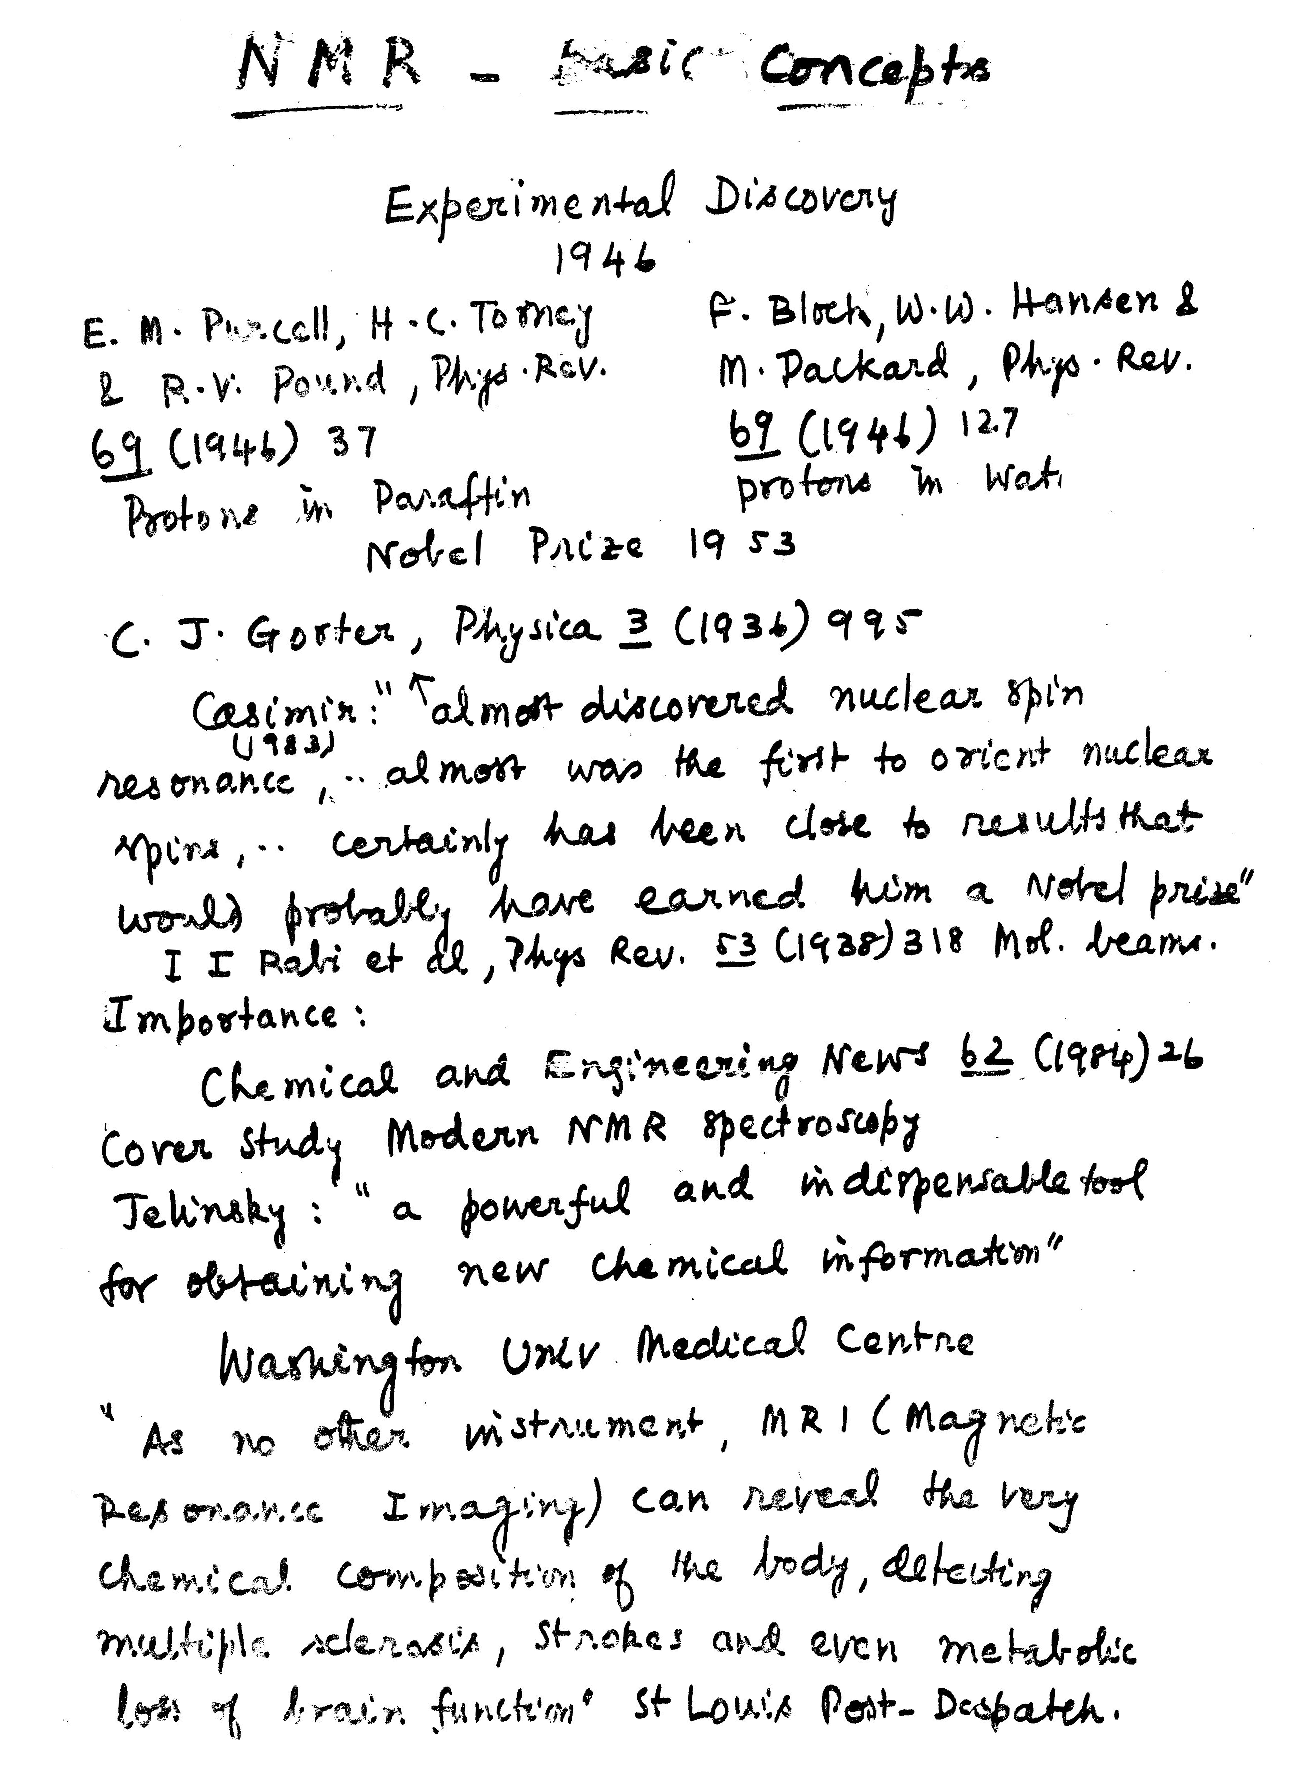
\includegraphics[scale=0.6]{src/images/chap8/1.eps}
\end{figure}
\begin{figure}[H]
\centering
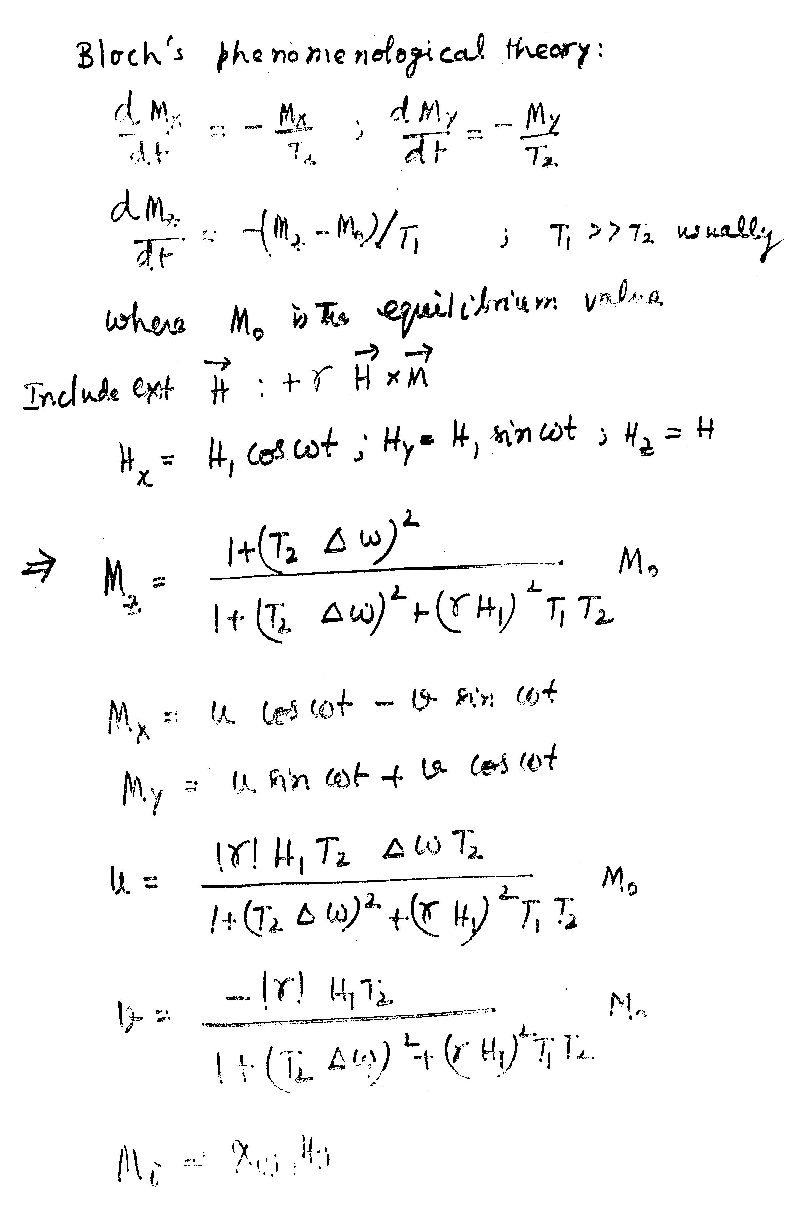
\includegraphics[scale=0.48]{src/images/chap8/2.eps}
\end{figure}
\begin{figure}[H]
\centering
\includegraphics[scale=0.485]{src/images/chap8/3.eps}
\end{figure}
\begin{figure}[H]
\centering
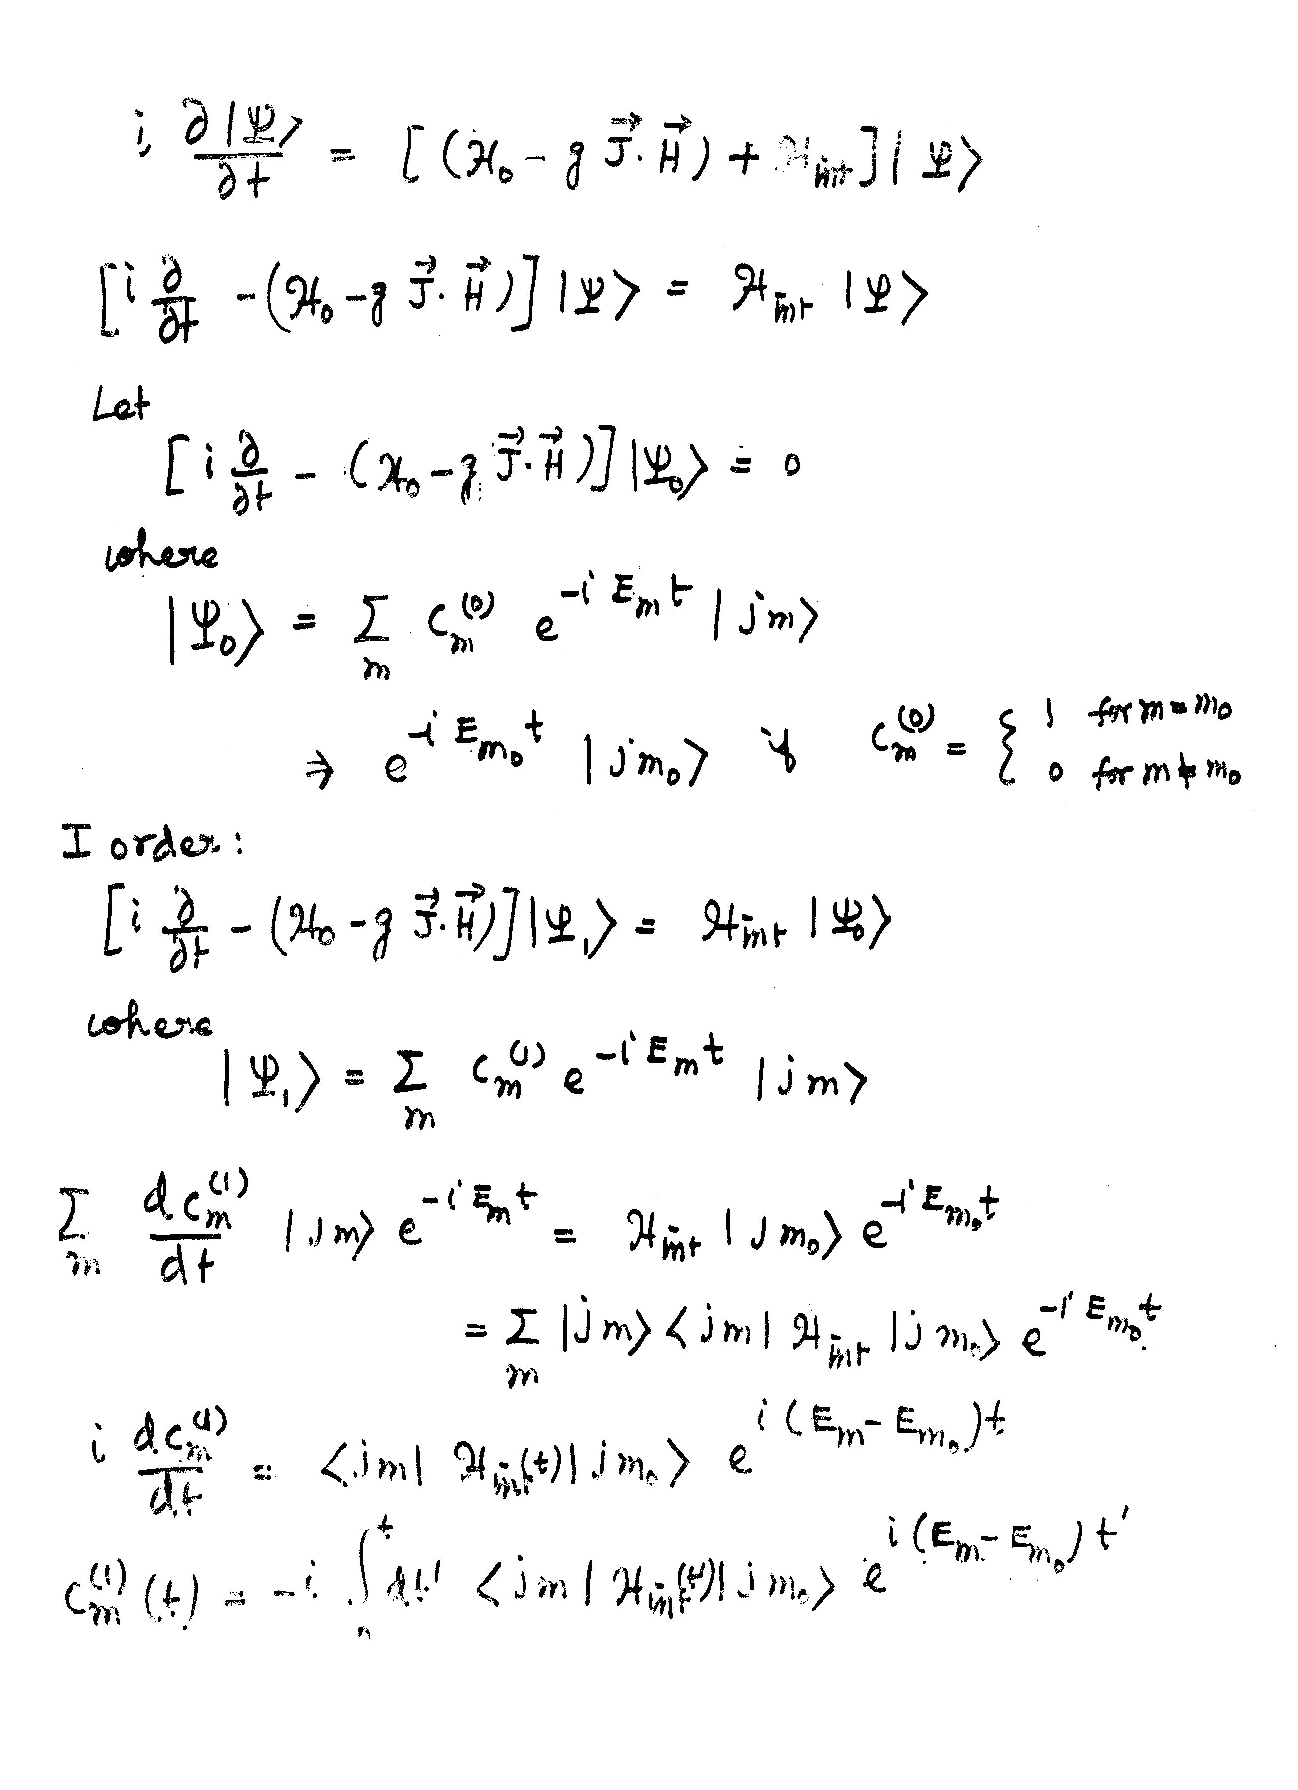
\includegraphics[scale=0.48]{src/images/chap8/4.eps}
\end{figure}
\begin{figure}[H]
\centering
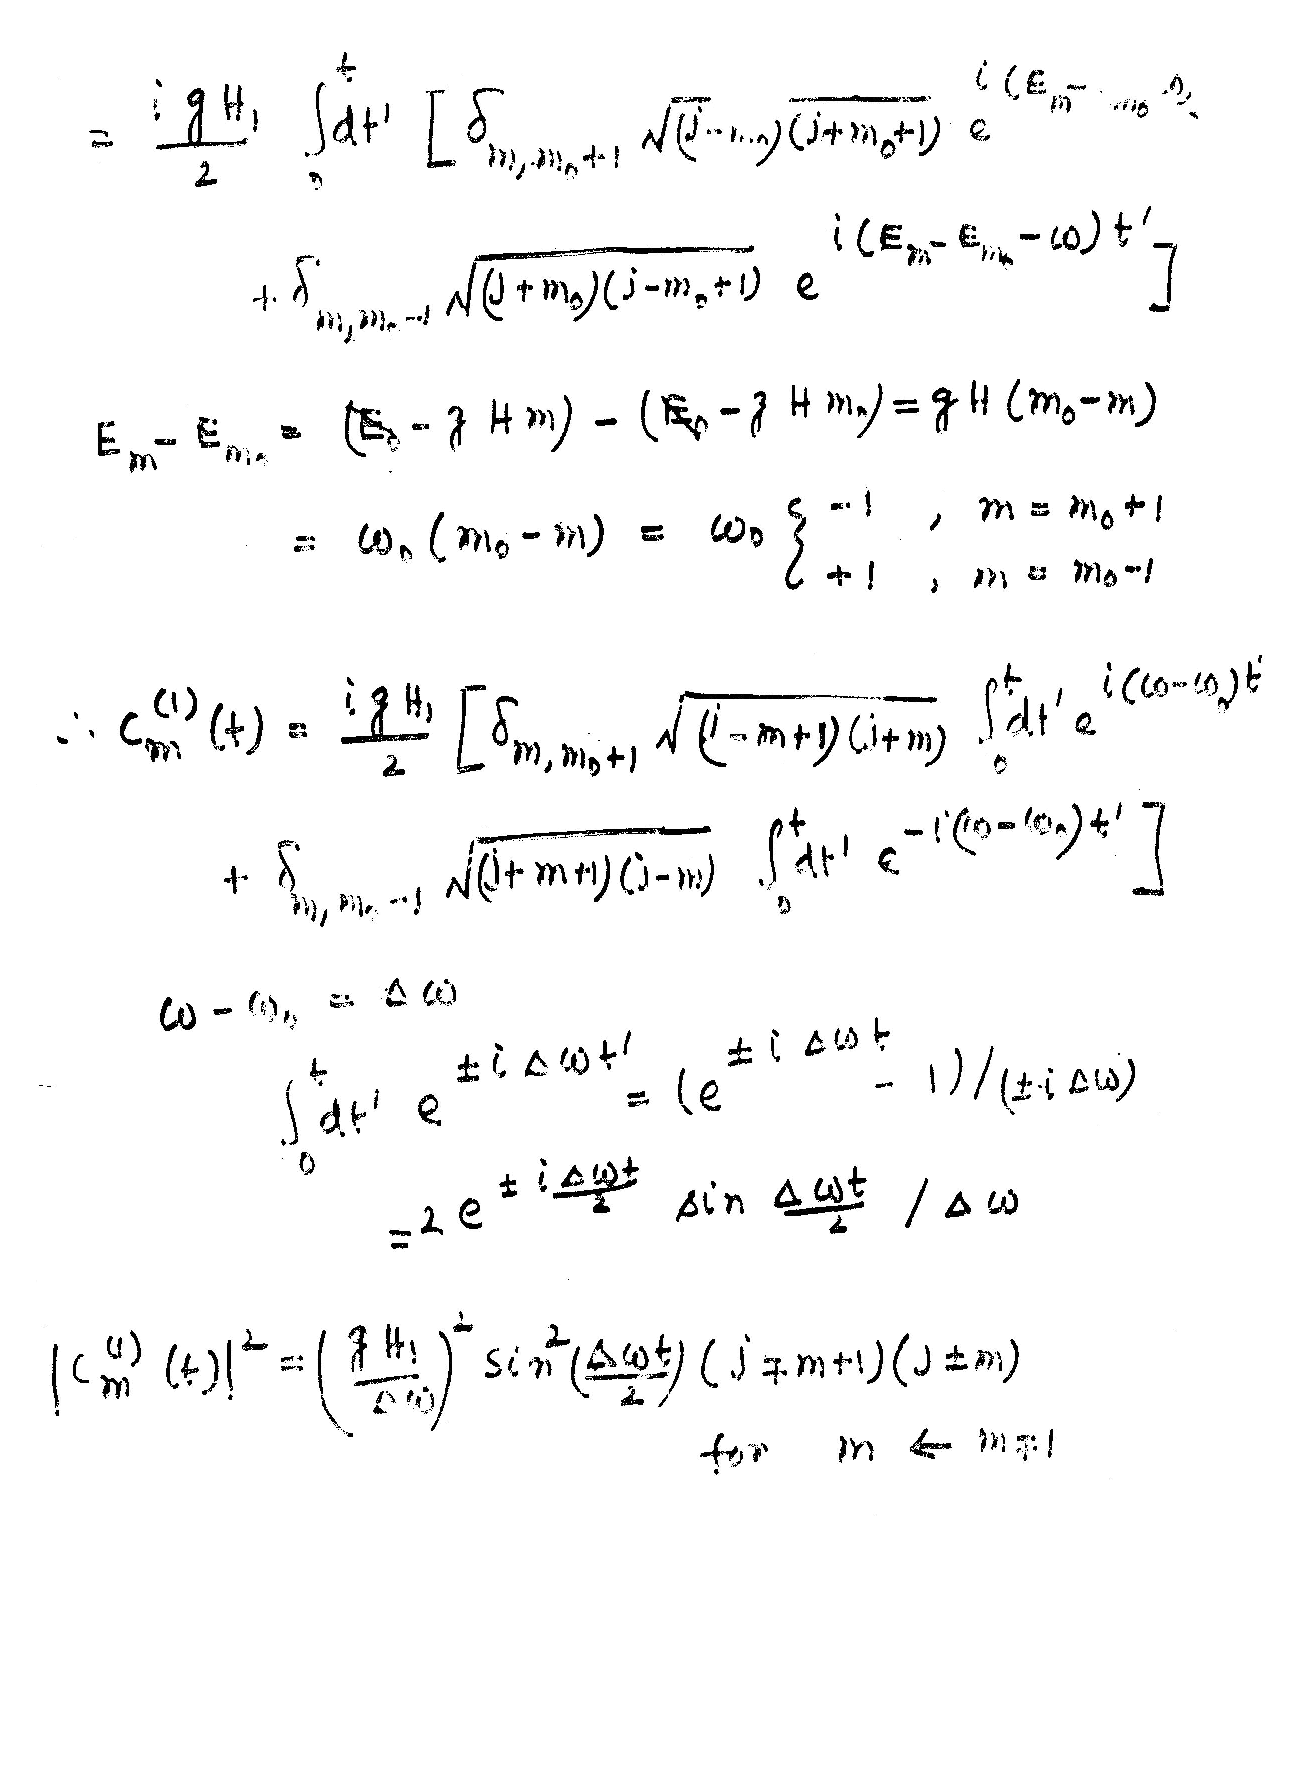
\includegraphics[scale=0.48]{src/images/chap8/5.eps}
\end{figure}
\begin{figure}[H]
\centering
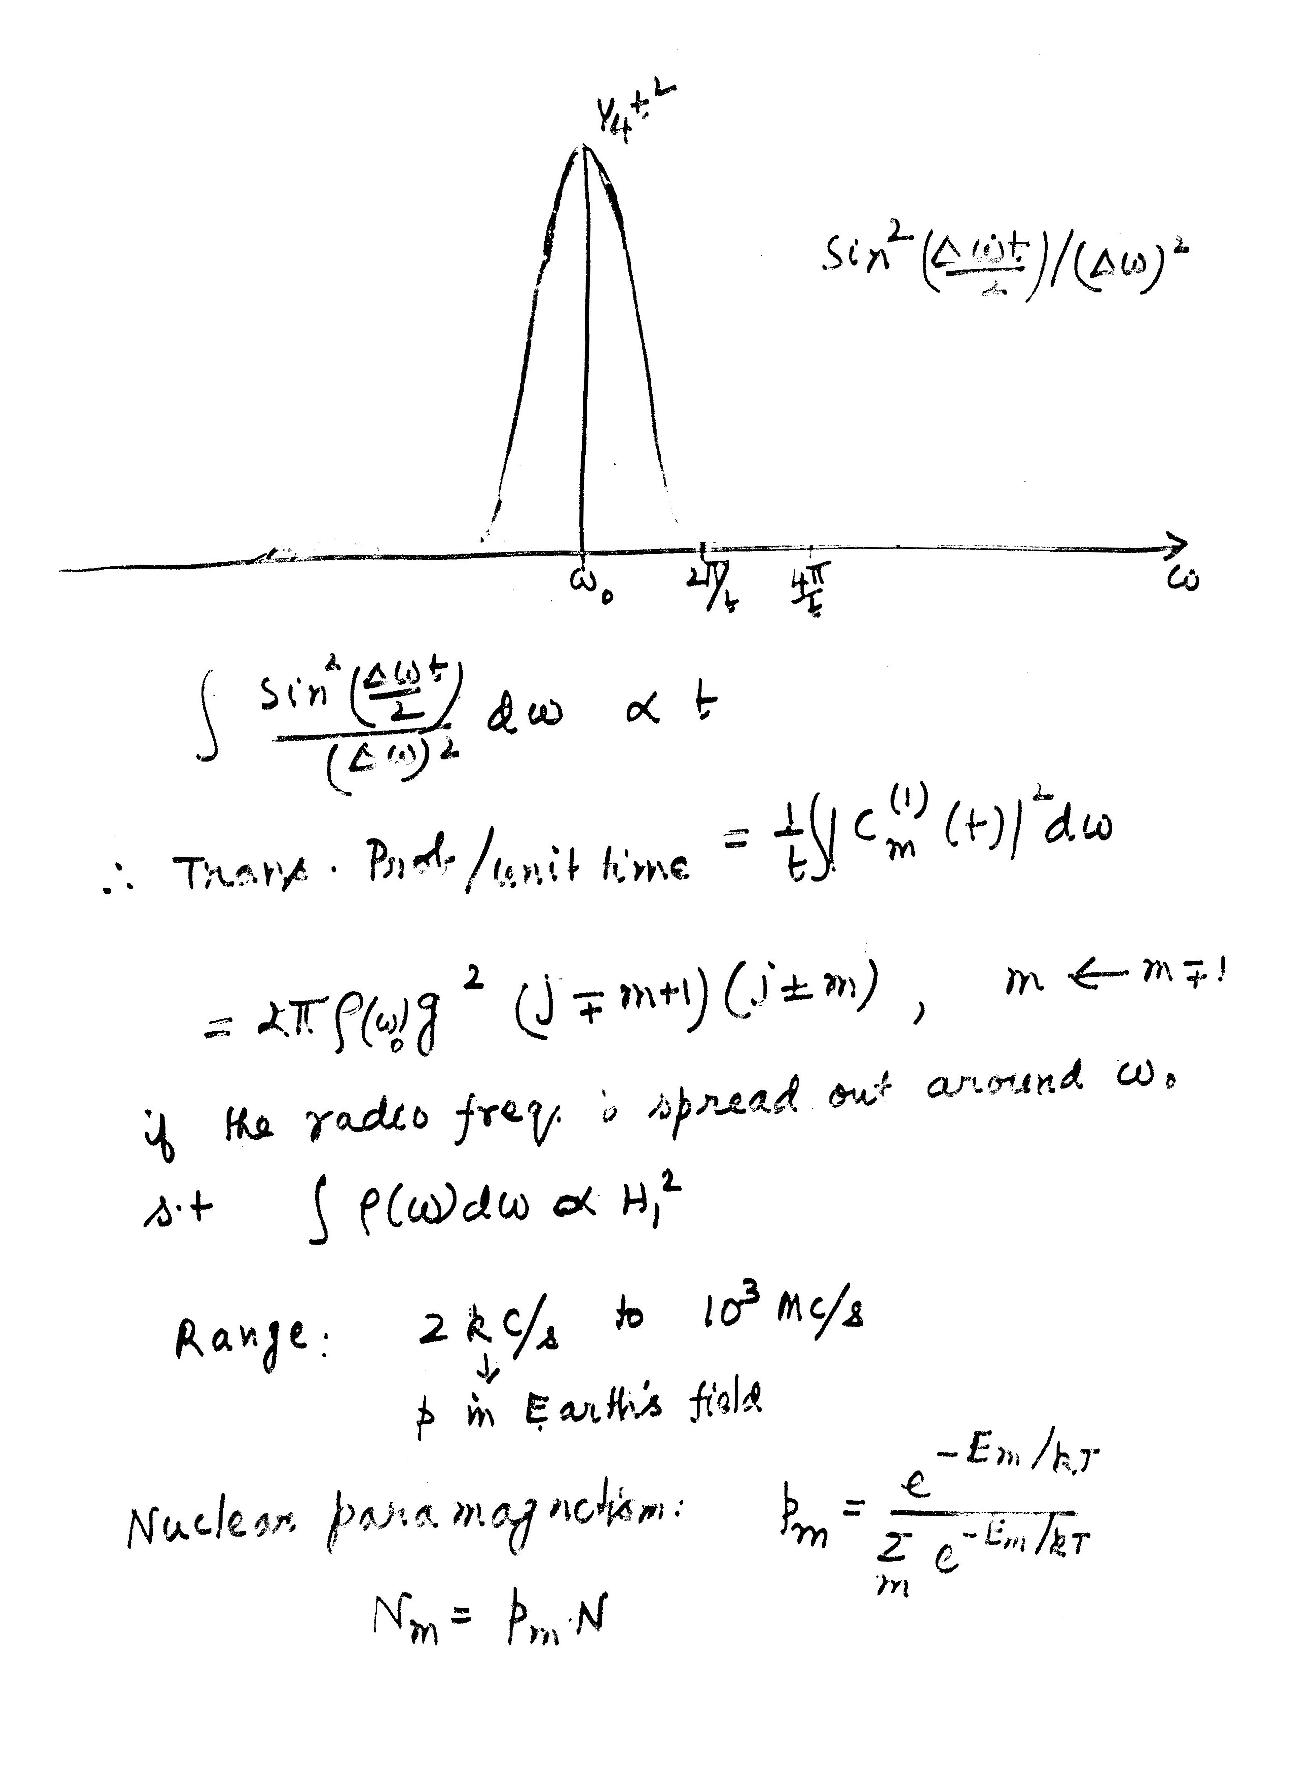
\includegraphics[scale=0.48]{src/images/chap8/6.eps}
\end{figure}
\begin{figure}[H]
\centering
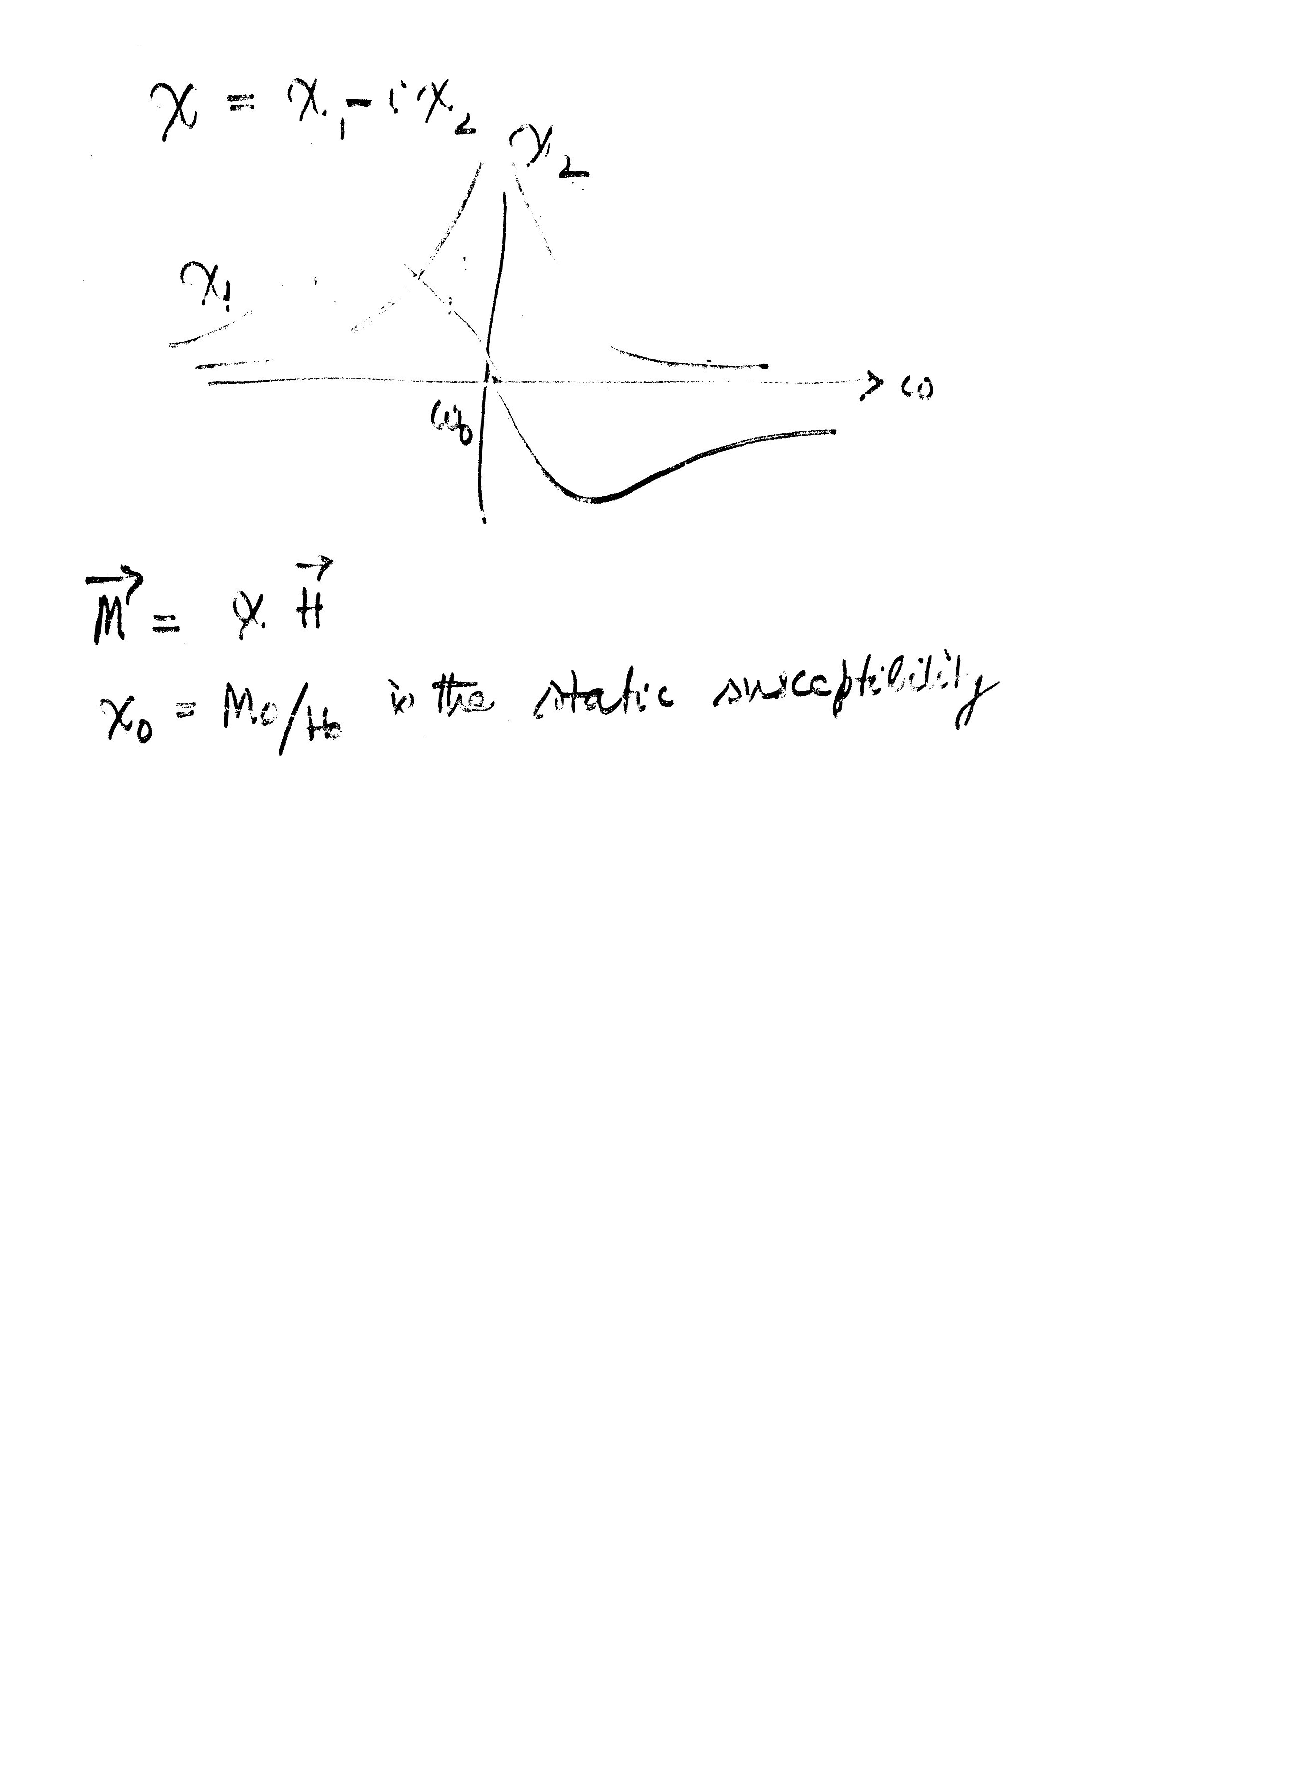
\includegraphics[scale=0.26]{src/images/chap8/7.eps}
\end{figure}
\vskip 1cm

\centerline{\includegraphics[scale=.8]{authorsphotos/Somasekhar.eps}}
\bigskip

\noindent
\textbf{Dr.\ R. Somasekhar} obtained the M.Sc.\ degree in 1975 and Ph.D. in 1982, both from Physics Department, Mysore University. 
He joined his Alma-Mater as a Lecturer in 1979 and retired from there, as Professor, in 2015. During this period he interacted closely with 
Prof.\ G. Ramachandran. Currently he leads an active retired life at Mysuru.
